\documentclass[13pt,oneside]{book}
\usepackage[utf8]{inputenc}
\usepackage{url}
\usepackage{graphicx}

\usepackage{geometry}
\geometry{a4paper, left=20mm, right=20mm, top=20mm, bottom=20mm}
\usepackage[margin=1.2in]{geometry}
\usepackage[toc,page]{appendix}
\usepackage{graphicx}
\usepackage{natbib}
\usepackage{lipsum}
\usepackage{caption}

\begin{document}

\captionsetup[figure]{margin=1.5cm,font=small,labelfont={bf},name={Figure},labelsep=colon,textfont={it}}
\captionsetup[table]{margin=1.5cm,font=small,labelfont={bf},name={Table},labelsep=colon,textfont={it}}
\setlipsumdefault{1}

\begin{titlepage}
\begin{center}
{\LARGE College Of Engineering Trivandrum}\\[3cm]
\linespread{1.2}\huge {\bfseries Application Software Development Lab}\\[3cm]
\linespread{1}

\includegraphics[width=5cm]{img/emblem.jpeg}\\[3cm]
{\Large Gokul K\\ S5  CSE \\ Roll No:21\\ TVE18CS021 }\\[1cm]


\textit{ }\\[2cm]
Department of Computer Science\\[0.2cm]
\today
\end{center}

\end{titlepage}

\newpage

\begin{frame}{}
    \centering
    \hspace*{-0.5cm}
    $\vcenter{\hbox{
\includegraphics[width=1.5cm]{img/emblem.jpeg}}}$
    $\vcenter{\resizebox{0.95\textwidth}{!}{
        \begin{tabular}{c}
             CS333 - Application Software Development Lab $\cdot$ 2020 $\cdot$   \\
             \hline 
        \end{tabular}
    }}$
\end{frame}
\section*{Cycle 1}
\section*{Expt 1}
\begin{center}
    \Large{Basic SQL Queries - I}
\end{center}

\section*{Aim}
\large{Creation of a database using DDL commands
	\begin{enumerate}
		\item Create Table
		\item Alter Table
		\item Truncate Table
		\item Drop Table
	\end{enumerate}
}

\section*{Experiment}
	\begin{enumerate}
		\item 
			Create a table named EMPLOYEE \\
			Syntax:
			\begin{verbatim}
				CREATE TABLE EMPLOYEE (
					EMPNO INTEGER(4) PRIMARY KEY,
					ENAME VARCHAR(10),
					DESIGNATION VARCHAR(10),
					SALARY DECIMAL(8, 2)
				);
				DESC EMPLOYEE;
			\end{verbatim}
			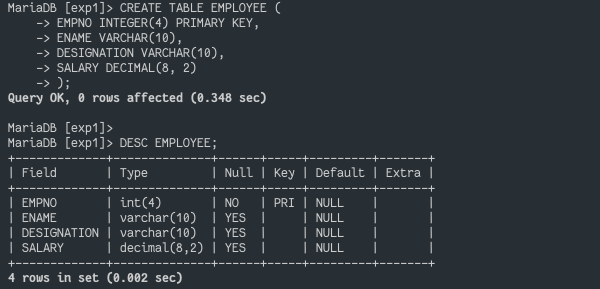
\includegraphics{img/p1/ss1.png}
		
			\item 
			a) Alter the table by adding column QUALIFICATION. \\
			b) Alter the table by modifying the EMPNO size to 6. \\
			c) Rename the table EMPLOYEE to EMP\_NEW. \\
			d) Drop the column QUALIFICATION.\\
			Syntax:
			\begin{verbatim}
				ALTER TABLE EMPLOYEE
				ADD QUALIFICATION VARCHAR(10);

				DESC EMPLOYEE;
			\end{verbatim}
			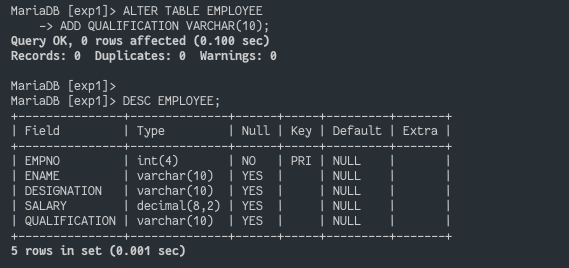
\includegraphics{img/p1/ss2.png}
			\begin{verbatim}
				ALTER TABLE EMPLOYEE
				MODIFY COLUMN EMPNO INTEGER(6);

				DESC EMPLOYEE;
			\end{verbatim}
			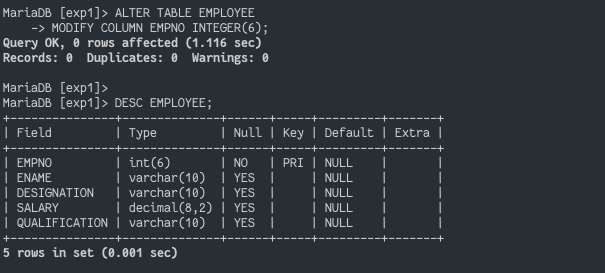
\includegraphics{img/p1/ss3.png}
			\begin{verbatim}
				ALTER TABLE EMPLOYEERENAME TO EMP_NEW;			
				DESC EMP_NEW;
			\end{verbatim}
			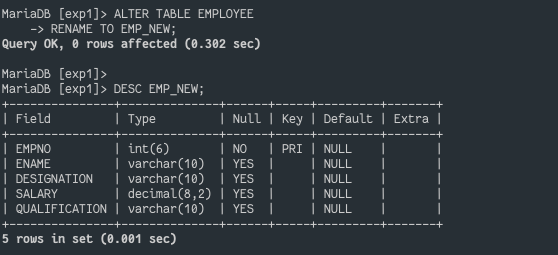
\includegraphics{img/p1/ss4.png}
			\begin{verbatim}
				ALTER TABLE EMP\_NEW
				DROP COLUMN QUALIFICATION;

				DESC EMP_NEW;
			\end{verbatim}
			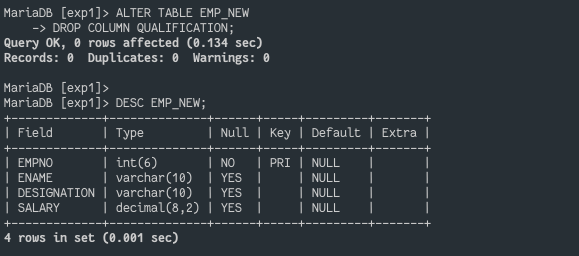
\includegraphics{img/p1/ss5.png}
		
		\item Truncate the table EMP\_NEW \\
		Syntax: 
		\begin{verbatim}
			INSERT INTO EMP_NEW 
			VALUES (1, "Name1", "Manager", 2000.00);

			SELECT * FROM EMP_NEW;

			TRUNCATE TABLE EMPLOYEE;

			SELECT * FROM EMP_NEW;
		\end{verbatim}
		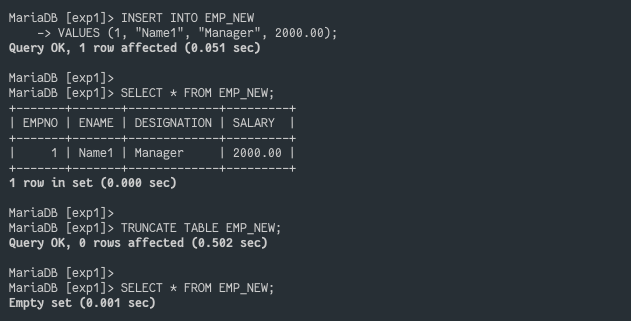
\includegraphics{img/p1/ss6.png}

		\item Drop the table \\
		Syntax: 
		\begin{verbatim}
			DROP TABLE EMP_NEW;

			DESC EMP_NEW;
		\end{verbatim}
		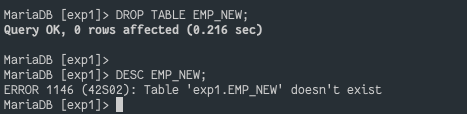
\includegraphics{img/p1/ss7.png}
	\end{enumerate}

	\section*{Result}
	The basic SQL for creating and modifying a table is executed and their output
	is verified
\end{document}